\documentclass{beamer}
\usetheme{Madrid}

\usepackage{amsmath, amssymb, amsthm}
\usepackage{graphicx}
\usepackage{listings}
\usepackage{gensymb}
\usepackage[utf8]{inputenc}
\usepackage{hyperref}
\usepackage{gvv}

\lstnewenvironment{ccode}
{\lstset{language=C, basicstyle=\small\ttfamily, breaklines=true, frame=single}}
{}

\begin{document}

\title{DISCRETE ASSIGNMENT}
\author{EE23BTECH11016 - Aditi Dure$^{*}$}
\date{}
\frame{\titlepage}

\begin{frame}
\frametitle{Question}
Consider the sequence whose $n^\text{th}$ term is given by \(2^n\). Find the first 6 terms of this sequence. \hfill(NCERT)
\end{frame}

\begin{frame}{allowframebreaks}
\frametitle{Solution: Theory}
\begin{table}[!ht]
    \centering
        \begin{tabular}{|c|c|c|} 
      \hline
\textbf{Variable}& \textbf{Description}& \textbf{Value}\\\hline
         $x(n)$& general term of sequence&$2^{n} u(n)$\\\hline
         
    \end{tabular}

    \caption{input parameters}
    \label{tab:11_9_1_3}
\end{table}
\end{frame}

\begin{frame}
\frametitle{Theory}

\begin{align}
X(Z) &= \frac {1}{1 - 2  z^{-1} } \quad \abs{z}>\abs{2}
\end{align}

\end{frame}

\begin{frame}
\frametitle{Theory}
 
\begin{figure}[H]
    \centering
    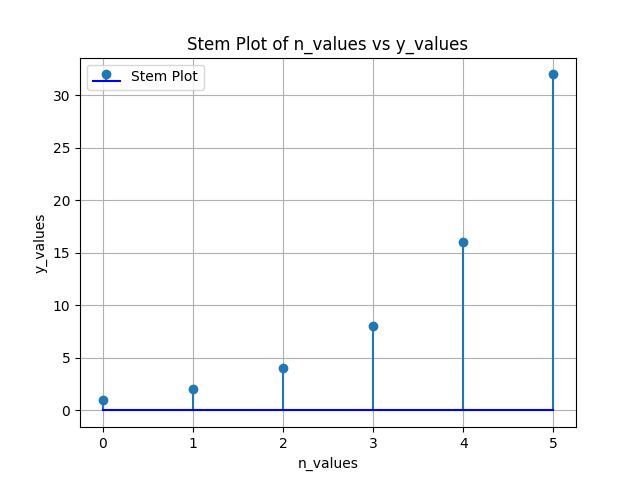
\includegraphics[width=0.5\textwidth]{figs/fig1.png}
    \caption{Six terms of the given sequence}
    \label{fig:11_9_1_3}
\end{figure}
\end{frame}

\begin{frame}[fragile]
\frametitle{Code: C}

\begin{lstlisting}[language=C, basicstyle=\small\ttfamily, breaklines=true, frame=single]
#include <stdio.h>
#include <math.h>

void linespace(int start, int stop, int step, int* n_values, int* y_values, int num_values) {
    for (int i = 0; i < num_values; ++i) {
        n_values[i] = start + i * step;
        y_values[i] = (int)pow(2, n_values[i]); // Adjust this line based on your specific calculation
    }
}
\end{lstlisting}
\end{frame}

\begin{frame}[fragile]
\frametitle{Code: C}
\begin{lstlisting}
int main() {
    // Define the range and step size
    int start = 0;
    int stop = 5;
    int step = 1;

    // Calculate the number of values in the range
    int num_values = (stop - start) / step + 1;

    // Allocate arrays to store the generated values
    int n_values[num_values];
    int y_values[num_values];

    // Call the linespace function
    linespace(start, stop, step, n_values, y_values, num_values);
\end{lstlisting}
\end{frame}

\begin{frame}[fragile]
\frametitle{Code: C}
\begin{lstlisting}
    // Save data to a file
    FILE* file = fopen("output.dat", "w");

    if (file != NULL) {
        for (int i = 0; i < num_values; ++i) {
            fprintf(file, "%d %d\n", n_values[i], y_values[i]);
        }

        fclose(file);
        printf("Data saved to 'output.dat'.\n");
    } else {
        printf("Error opening file for writing.\n");
    }

    return 0;
}
\end{lstlisting}
\end{frame}

\begin{frame}[fragile]
\frametitle{Code: Python}
\begin{lstlisting}[language=Python, basicstyle=\small\ttfamily, breaklines=true, frame=single]
import matplotlib.pyplot as plt
import numpy as np

# Load data from the "output.dat" file using numpy's loadtxt
data = np.loadtxt("output.dat")

# Extract n_values and y_values from the data
n_values = data[:, 0].astype(int)
y_values = data[:, 1].astype(int)

\end{lstlisting}
\end{frame}
\begin{frame}[fragile]
\frametitle{Code: Python}
\begin{lstlisting}

# Create a stem plot
plt.stem(n_values, y_values, linefmt='|', markerfmt='o', basefmt='b', label='Stem Plot')

plt.xlabel('n_values')
plt.ylabel('y_values')
plt.title('Stem Plot of n_values vs y_values')
plt.grid(True)
plt.legend()

plt.savefig('figs/fig1.png')
\end{lstlisting}
\end{frame}

\end{document}

